% Gemini theme
% https://github.com/anishathalye/gemini

\documentclass[final]{beamer}

% ====================
% Packages
% ====================

\usepackage[T1]{fontenc}
\usepackage{lmodern}
\usepackage[size=custom,width=120,height=106.68,scale=1.2]{beamerposter}
\usetheme{gemini}
\usecolortheme{gemini}
\usepackage{graphicx}
\usepackage{booktabs}
\usepackage{tikz}
\usepackage{svg}
\usepackage{pgfplots}
\pgfplotsset{compat=1.14}
\usepackage{anyfontsize}
\usepackage{siunitx}
\usepackage{multicol}
\usepackage{physics}
\usepackage{bm}
\AtBeginDocument{\RenewCommandCopy\qty\SI}

% ====================
% Lengths
% ====================

% If you have N columns, choose \sepwidth and \colwidth such that
% (N+1)*\sepwidth + N*\colwidth = \paperwidth
\newlength{\sepwidth}
\newlength{\colwidth}
\setlength{\sepwidth}{0.025\paperwidth}
\setlength{\colwidth}{0.3\paperwidth} 

\newcommand{\separatorcolumn}{\begin{column}{\sepwidth}\end{column}}

% ====================
% Title
% ====================

\title{MIDSX: A Monte Carlo Interaction and Dosimetry Simulation of X-rays}

\author{John Meneghini}

\institute[shortinst]{Department of Physics, Saint Vincent College, Latrobe, PA 15650}

% ====================
% Footer (optional)
% ====================

\footercontent{
  \href{https://www.example.com}{https://www.example.com} \hfill
  ABC Conference 2025, New York --- XYZ-1234 \hfill
  \href{mailto:alyssa.p.hacker@example.com}{alyssa.p.hacker@example.com}}
% (can be left out to remove footer)

% ====================
% Logo (optional)
% ====================

% use this to include logos on the left and/or right side of the header:
% \logoright{\includegraphics[height=7cm]{logo1.pdf}}
\logoleft{
\includegraphics[height=7cm]{svc_logo.pdf}}

% ====================
% Body
% ====================

\begin{document}

\begin{frame}[t]
\begin{columns}[t]
\separatorcolumn

\begin{column}{\colwidth}

  \begin{block}{Introduction}
    \begin{itemize}
      \item Computed Tomography (CT) imaging is crucial in medical diagnostics but involves risks from ionizing radiation.
      \item Monitoring of radiation exposure is essential, measured in absorbed dose and air kerma.
      \item Monte Carlo (MC) methods allow for precise radiation exposure estimation through accurate photon interaction simulations.
      \item This poster introduces MIDSX, an open-source MC photon transport code system optimized for x-ray transport in medical imaging.
      \item MIDSX's focused design reduces the complexity of implementation and has been validated against established
      benchmarks, showing its diagnostic potential.
    \end{itemize}
  
  \end{block}

  \begin{block}{Simulation Geometry}
    The geometry of a transport simulation consists of the following objects:
    \begin{itemize}
      \item A source object to specify the generation of photons.
      \item Voxel grid(s), stored via NifTI files, to contain object/body geometries and material information.
      \item Tally(s) to track trajectories of photons, incident energy, deposited energy, and other quantities of interest.
      \item A computational domain to contain these objects and to specify a background material.
    \end{itemize}

    \begin{figure}
      \centering
      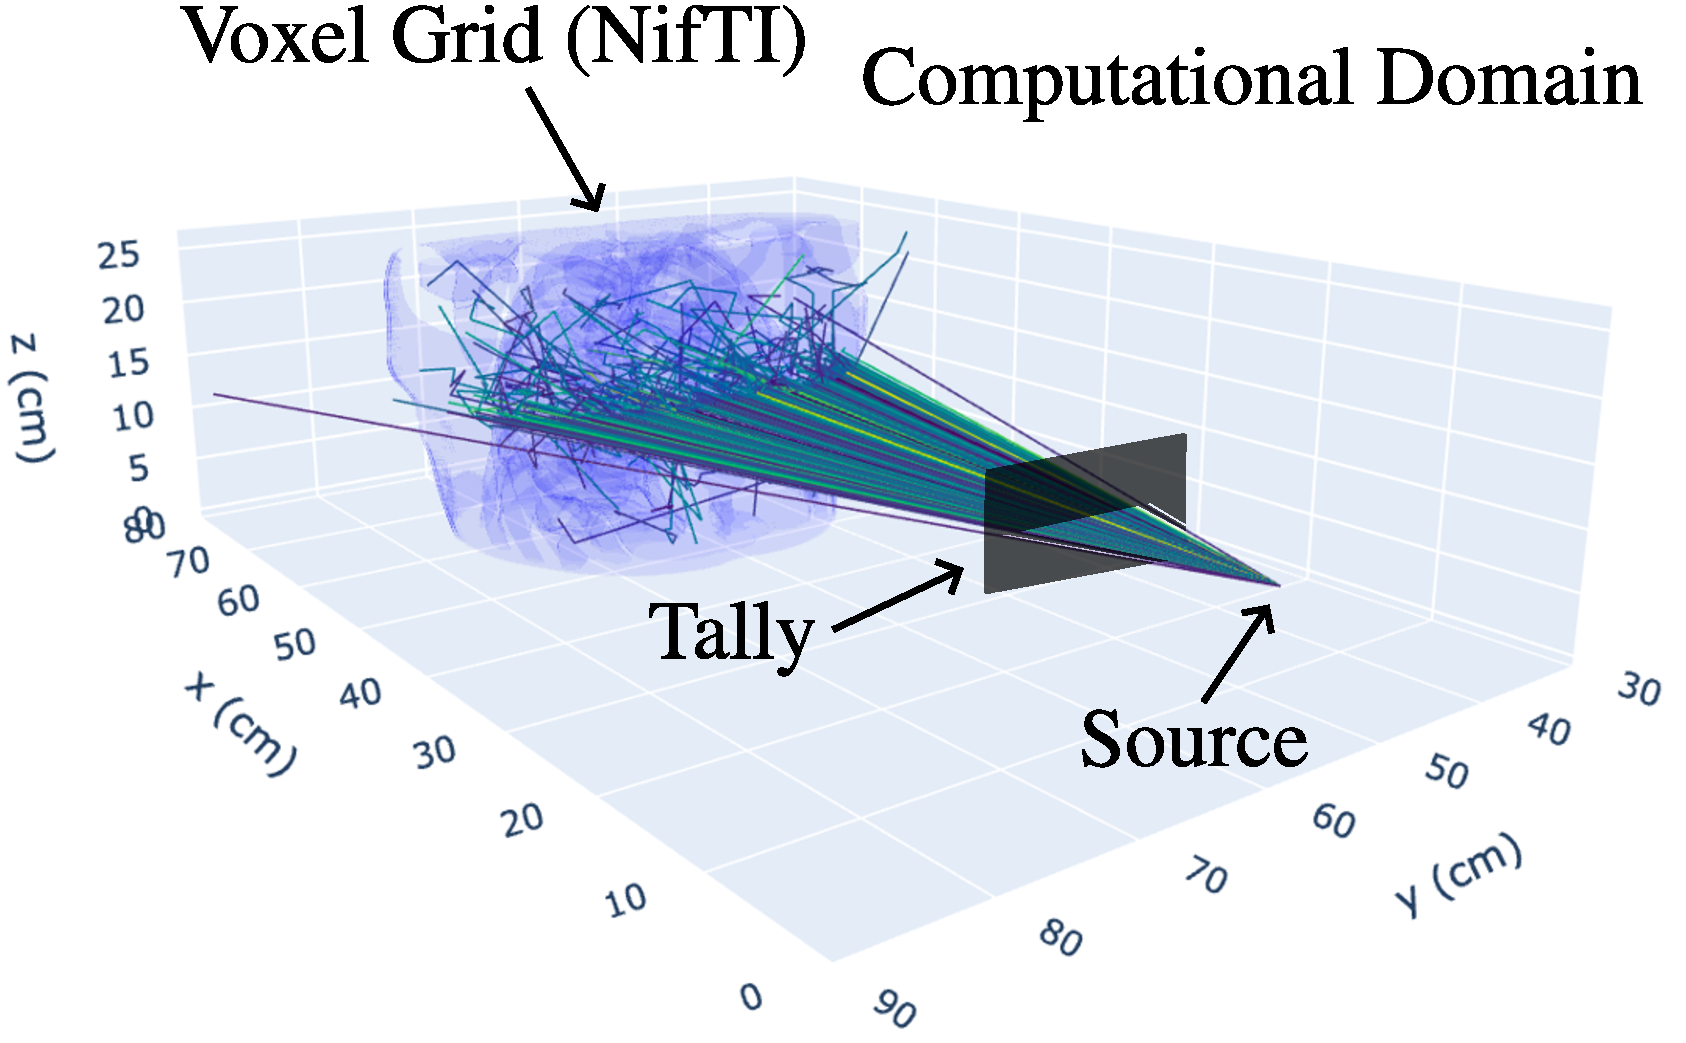
\includegraphics[width = \colwidth]{comp_domain.pdf}
      \caption{A typical transport geometry used in MIDSX.}
    \end{figure}
    

  \end{block}

  \begin{block}{Transport Theory}

    \begin{itemize}
      \item As a photon take "steps" through a homogenous computational domain, its position after taking the $n$-th step is represented by the parametric ray equation:
    \end{itemize}
    \begin{equation} \label{eq:r_n}
        \va{r}_{\bm{n}} = \va{r}_{\bm{n-1}} + \vu{d}t,
    \end{equation}
    where $\va{r}_{\bm{n-1}}$ is the position before the $n$-th step, $\vu{d}$ is a unit vector in the direction of the step, and $t$ is the length of the $n$-th step.
    \begin{itemize}
      \item For a photon of energy $E$ in material $M$, MIDSX randomly samples $t$ for use in Eq.~\ref{eq:r_n} from the following probability distribution function (PDF):
    \end{itemize}
    \begin{equation} \label{eq:pdf}
      p(t) = n\sigma \exp\left[-t(n\sigma)\right],
    \end{equation}
    where $n$ is the number density of $M$ and $\sigma = \sigma(E, M)$ is the microscopic cross-section of $M$ at $E$.
    \begin{itemize}
      \item Using the inversion method for sampling a PDF on Eq.~\ref{eq:pdf}, random values of $t$ can be generated from
    \end{itemize}
    \begin{equation} \label{eq:t_inv}
      t = -\frac{1}{n\sigma} \ln \gamma, 
    \end{equation}
    where $\gamma$ is a uniformly distributed random number in the interval $[0, 1)$.
  \end{block}

\end{column}

\separatorcolumn

\begin{column}{\colwidth}

  % continuing theory, so no new block
  \begin{itemize}
    \item In order to generalize this to an inhomogeneous domain, MIDSX uses $\delta$ tracking.
    \item This effectively changes $\sigma \rightarrow \sigma_{\rm{max}}$ in Eq.~\ref{eq:pdf} and Eq.~\ref{eq:t_inv}, where $\sigma_{\rm{max}}$ is the maximum cross-section in the domain.
    \item In order to correct for the resulting systematic decrease in $t$, we implement $\delta$ interactions as an alternative to photon-matter interactions. The probability of which is given by 
  \end{itemize}
  \begin{equation}
    P_{\delta} = \frac{\sigma_{\text{max}}(E) - \sigma(E, M)}{\sigma_{\text{max}}(E)}.
  \end{equation}


  \begin{block}{Photon-Matter Interactions}
    There are 3 fundamental possible photon-matter interactions in the medical x-ray energy range:
    \begin{center}
      \textbf{Common Variables}
    \end{center}

    \begin{multicols}{2}
      \begin{center}
        $E$ - Energy of incoming photon\\
        $\theta_e$ - Angle of ejected electron\\
        \vspace{\baselineskip}
        \textbf{1. Photoelectric Effect}
      \begin{itemize}
        \item Photon interacts with electron of target atom, resulting in an electron being ejected with $E_e = E - U_i$ and the photon being absorbed.
      \end{itemize}
      \end{center}
      \vfill
      \begin{figure}
        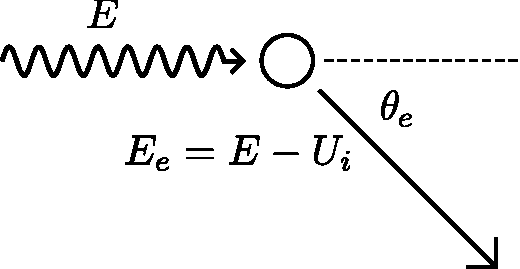
\includegraphics[width = 0.4\colwidth]{photoelectric_diagram.pdf}
        \caption{A diagram representing the photoelectric effect.}
      \end{figure}
      \columnbreak%
      \begin{center}
        $\theta$ - Angle of scattered photon \\
        $U_i$ - Binding energy of subshell\\
        \vspace{\baselineskip}
        \textbf{2. Compton Scattering}
      \begin{itemize}
        \item Photon interacts with electron of target atom, resulting in a scattered photon of energy $E'$ and a released electron with energy $E_e = E - E' - U_i$.
      \end{itemize}
      \end{center}
      \begin{figure}
        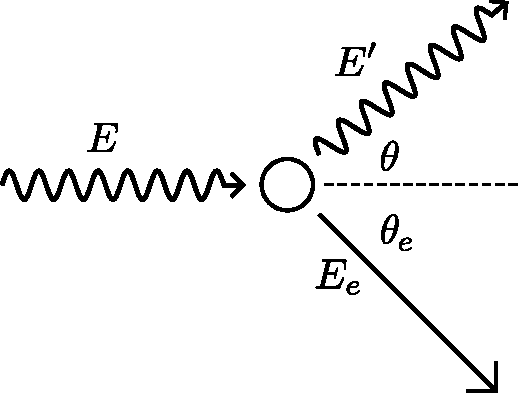
\includegraphics[width = 0.4\colwidth]{compton_diagram.pdf}
        \caption{A diagram representing Rayleigh scattering.}
      \end{figure}

    \end{multicols}

    \begin{center}
      \textbf{3. Rayleigh Scattering}
      \begin{itemize}
        \item Photon interacts coherently with atom, resulting in photon scattering with no energy loss.
      \end{itemize}
      \vspace{-2\baselineskip}
      \begin{figure}
        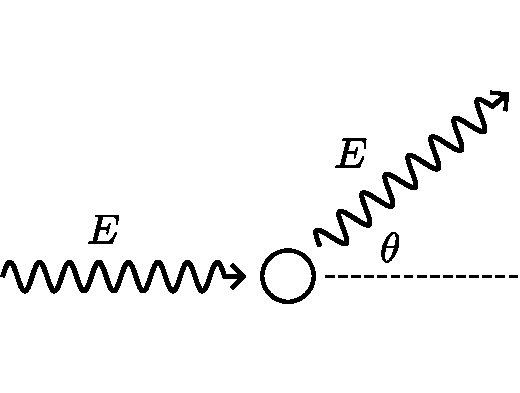
\includegraphics[width = 0.4\colwidth]{rayleigh_diagram.pdf}
        \caption{A diagram representing Compton scattering.}
      \end{figure}
    \end{center}


  \end{block}

  \begin{block}{Fusce aliquam magna velit}

    Et rutrum ex euismod vel. Pellentesque ultricies, velit in fermentum
    vestibulum, lectus nisi pretium nibh, sit amet aliquam lectus augue vel
    velit. Suspendisse rhoncus massa porttitor augue feugiat molestie. Sed
    molestie ut orci nec malesuada. Sed ultricies feugiat est fringilla
    posuere.

    \begin{figure}
      \centering
      \begin{tikzpicture}
        \begin{axis}[
            scale only axis,
            no markers,
            domain=0:2*pi,
            samples=100,
            axis lines=center,
            axis line style={-},
            ticks=none]
          \addplot[red] {sin(deg(x))};
          \addplot[blue] {cos(deg(x))};
        \end{axis}
      \end{tikzpicture}
      \caption{Another figure caption.}
    \end{figure}

  \end{block}

  \begin{block}{Nam cursus consequat egestas}

    Nulla eget sem quam. Ut aliquam volutpat nisi vestibulum convallis. Nunc a
    lectus et eros facilisis hendrerit eu non urna. Interdum et malesuada fames
    ac ante \textit{ipsum primis} in faucibus. Etiam sit amet velit eget sem
    euismod tristique. Praesent enim erat, porta vel mattis sed, pharetra sed
    ipsum. Morbi commodo condimentum massa, \textit{tempus venenatis} massa
    hendrerit quis. Maecenas sed porta est. Praesent mollis interdum lectus,
    sit amet sollicitudin risus tincidunt non.

    Etiam sit amet tempus lorem, aliquet condimentum velit. Donec et nibh
    consequat, sagittis ex eget, dictum orci. Etiam quis semper ante. Ut eu
    mauris purus. Proin nec consectetur ligula. Mauris pretium molestie
    ullamcorper. Integer nisi neque, aliquet et odio non, sagittis porta justo.

    \begin{itemize}
      \item \textbf{Sed consequat} id ante vel efficitur. Praesent congue massa
        sed est scelerisque, elementum mollis augue iaculis.
        \begin{itemize}
          \item In sed est finibus, vulputate
            nunc gravida, pulvinar lorem. In maximus nunc dolor, sed auctor eros
            porttitor quis.
          \item Fusce ornare dignissim nisi. Nam sit amet risus vel lacus
            tempor tincidunt eu a arcu.
          \item Donec rhoncus vestibulum erat, quis aliquam leo
            gravida egestas.
        \end{itemize}
      \item \textbf{Sed luctus, elit sit amet} dictum maximus, diam dolor
        faucibus purus, sed lobortis justo erat id turpis.
      \item \textbf{Pellentesque facilisis dolor in leo} bibendum congue.
        Maecenas congue finibus justo, vitae eleifend urna facilisis at.
    \end{itemize}

  \end{block}

\end{column}

\separatorcolumn

\begin{column}{\colwidth}

  \begin{exampleblock}{A highlighted block containing some math}

    A different kind of highlighted block.

    $$
    \int_{-\infty}^{\infty} e^{-x^2}\,dx = \sqrt{\pi}
    $$

    Interdum et malesuada fames $\{1, 4, 9, \ldots\}$ ac ante ipsum primis in
    faucibus. Cras eleifend dolor eu nulla suscipit suscipit. Sed lobortis non
    felis id vulputate.

    \heading{A heading inside a block}

    Praesent consectetur mi $x^2 + y^2$ metus, nec vestibulum justo viverra
    nec. Proin eget nulla pretium, egestas magna aliquam, mollis neque. Vivamus
    dictum $\mathbf{u}^\intercal\mathbf{v}$ sagittis odio, vel porta erat
    congue sed. Maecenas ut dolor quis arcu auctor porttitor.

    \heading{Another heading inside a block}

    Sed augue erat, scelerisque a purus ultricies, placerat porttitor neque.
    Donec $P(y \mid x)$ fermentum consectetur $\nabla_x P(y \mid x)$ sapien
    sagittis egestas. Duis eget leo euismod nunc viverra imperdiet nec id
    justo.

  \end{exampleblock}

  \begin{block}{Nullam vel erat at velit convallis laoreet}

    Class aptent taciti sociosqu ad litora torquent per conubia nostra, per
    inceptos himenaeos. Phasellus libero enim, gravida sed erat sit amet,
    scelerisque congue diam. Fusce dapibus dui ut augue pulvinar iaculis.

    \begin{table}
      \centering
      \begin{tabular}{l r r c}
        \toprule
        \textbf{First column} & \textbf{Second column} & \textbf{Third column} & \textbf{Fourth} \\
        \midrule
        Foo & 13.37 & 384,394 & $\alpha$ \\
        Bar & 2.17 & 1,392 & $\beta$ \\
        Baz & 3.14 & 83,742 & $\delta$ \\
        Qux & 7.59 & 974 & $\gamma$ \\
        \bottomrule
      \end{tabular}
      \caption{A table caption.}
    \end{table}

    Donec quis posuere ligula. Nunc feugiat elit a mi malesuada consequat. Sed
    imperdiet augue ac nibh aliquet tristique. Aenean eu tortor vulputate,
    eleifend lorem in, dictum urna. Proin auctor ante in augue tincidunt
    tempor. Proin pellentesque vulputate odio, ac gravida nulla posuere
    efficitur. Aenean at velit vel dolor blandit molestie. Mauris laoreet
    commodo quam, non luctus nibh ullamcorper in. Class aptent taciti sociosqu
    ad litora torquent per conubia nostra, per inceptos himenaeos.

    Nulla varius finibus volutpat. Mauris molestie lorem tincidunt, iaculis
    libero at, gravida ante. Phasellus at felis eu neque suscipit suscipit.
    Integer ullamcorper, dui nec pretium ornare, urna dolor consequat libero,
    in feugiat elit lorem euismod lacus. Pellentesque sit amet dolor mollis,
    auctor urna non, tempus sem.

  \end{block}

  \begin{block}{References}

    \nocite{*}
    \footnotesize{\bibliographystyle{plain}\bibliography{poster}}

  \end{block}

\end{column}

\separatorcolumn
\end{columns}
\end{frame}

\end{document}
